\documentclass[12pt]{amsart}
\usepackage[margin=1in]{geometry}
\usepackage{amssymb,amsfonts,amsmath}
\usepackage{color}
\usepackage{enumerate}
\usepackage{mathrsfs}
\usepackage{hyperref}
\usepackage[capitalise]{cleveref}
\usepackage{constants}
\usepackage{parskip}
\usepackage{indentfirst}
\usepackage{enumitem}
\usepackage{tikz}
\usepackage{graphicx}
\usepackage{longtable}
\usetikzlibrary{shapes.geometric, arrows}
\setlength{\parindent}{2em}
\hfuzz=200pt

%----Theorem Environments----
\newtheorem{theorem}{Theorem}[section]
\newtheorem{corollary}[theorem]{Corollary}
\newtheorem{hypothesis}[theorem]{Hypothesis}
\newtheorem{proposition}[theorem]{Proposition}
\newtheorem{lemma}[theorem]{Lemma}
\newtheorem{problem*}{Problem}

\theoremstyle{definition}
\newtheorem{definition}[theorem]{Definition}
\newtheorem{example}[theorem]{Example}
\newcommand{\exercise}[1]{\noindent {\bf Exercise #1.}}

\numberwithin{equation}{section}

\crefname{figure}{Figure}{Figures}
\crefname{theorem}{Theorem}{Theorems}
\crefname{cor}{Corollary}{Corollaries}
\crefname{exercise}{Exercise}{Exercises}
\crefname{cor*}{Corollary}{Corollaries}
\crefname{lem}{Lemma}{Lemmas}
\crefname{prop}{Proposition}{Propositions}
\crefname{conj}{Conjecture}{Conjectures}
\crefname{defn}{Definition}{Definitions}
\crefname{hyp}{Hypothesis}{Hypotheses}

\newcommand{\Z}{\mathbb{Z}}
\renewcommand{\C}{\mathbb{C}}
\newcommand{\R}{\mathbb{R}}
\newcommand{\Q}{\mathbb{Q}}
\newcommand{\F}{\mathbb{F}}
\newcommand{\N}{\mathbb{N}}
\newcommand{\re}{\textup{Re}}
\newcommand{\im}{\textup{Im}}
\renewcommand{\epsilon}{\varepsilon}
\newcommand{\Li}{\mathrm{Li}}

\title{Math 417, Homework 7}
\author{Charles Ancel}

\begin{document}
\maketitle

%-----------------------------
\begin{exercise}{1} Write \(Z = \{cI \ | \ c\in \R^x\}\) for the subgroup of non-zero multiples of the identity matrix in \(GL_n(\R)\). Show the following:

    \begin{enumerate}[label=\textbf{\alph*.}]
        \item If $n$ is odd, then \(SL_n(\R)Z=GL_n(\R)\) and \(SL_n(\R) \cap Z = \{I\}\), and therefore \(PGL_n(\R) \simeq SL_n(\R)\)
        \item If $n$ is even, then \(SL_n(\R)=GL^+_n(\R)\), the matrices $A$ with \(\det A > 0\), and that \(SL_n(\R) \cap Z = \{\pm  I\}\). Conclude that \(PGL_n(\R)\) contains an index 2 subgroup which is isomorphic to \(SL_n(\R)/ \{\pm I\}\).
    \end{enumerate}

    \noindent\rule{\linewidth}{1pt}
    
    \section*{Solution}

    \subsection*{a. \(SL_n(\R)Z=GL_n(\R)\) for odd \(n\)}

    Let \(A \in GL_n(\R)\). We need to show that \(A\) can be written as a product of an element in \(SL_n(\R)\) and an element in \(Z\).

    \begin{proof} \(\)

    Consider the matrix \(c^{-1}A\), where \(c = \det(A)^{1/n}\). Note that:
    \[
    \det(c^{-1}A) = c^{-n} \det(A) = (\det(A)^{1/n})^{-n} \det(A) = 1.
    \]
    Thus, \(c^{-1}A \in SL_n(\R)\).

    Therefore, \(A = (c^{-1}A) \cdot cI\), where \(c^{-1}A \in SL_n(\R)\) and \(cI \in Z\). This shows that \(A \in SL_n(\R)Z\). Since \(A \in GL_n(\R)\) was arbitrary, we have \(GL_n(\R) = SL_n(\R)Z\).

    Next, we need to show that \(SL_n(\R) \cap Z = \{I\}\).

    Let \(A \in SL_n(\R) \cap Z\). Then \(A = cI\) for some \(c \in \R^*\), and \(\det(A) = 1\). Thus,
    \[
    \det(cI) = c^n = 1.
    \]
    Since \(n\) is odd, \(c = 1\). Therefore, \(A = I\), and \(SL_n(\R) \cap Z = \{I\}\).

    Hence, \(PGL_n(\R) = GL_n(\R) / Z \cong SL_n(\R)\).

    \end{proof}

    \subsection*{b. \(SL_n(\R) = GL^+_n(\R)\) for even \(n\)}

    Let \(n\) be even. We need to show that \(SL_n(\R) = GL^+_n(\R)\), the group of matrices \(A \in GL_n(\R)\) with \(\det A > 0\).

    \begin{proof} \(\)

    Consider any matrix \(A \in GL^+_n(\R)\). We need to show that \(A\) can be written as a product of an element in \(SL_n(\R)\) and an element in \(Z\).

    Let \(c = \det(A)^{1/n}\). Then \(c > 0\), and consider the matrix \(c^{-1}A\). We have:
    \[
    \det(c^{-1}A) = c^{-n} \det(A) = (\det(A)^{1/n})^{-n} \det(A) = 1.
    \]
    Thus, \(c^{-1}A \in SL_n(\R)\).

    Therefore, \(A = (c^{-1}A) \cdot cI\), where \(c^{-1}A \in SL_n(\R)\) and \(cI \in Z\). This shows that \(A \in SL_n(\R)Z\). Since \(A \in GL^+_n(\R)\) was arbitrary, we have \(GL^+_n(\R) = SL_n(\R)Z\).

    Next, we need to show that \(SL_n(\R) \cap Z = \{\pm I\}\).

    Let \(A \in SL_n(\R) \cap Z\). Then \(A = cI\) for some \(c \in \R^*\), and \(\det(A) = 1\). Thus,
    \[
    \det(cI) = c^n = 1.
    \]
    Since \(n\) is even, \(c^n = 1\) implies \(c = \pm 1\). Therefore, \(A = I\) or \(A = -I\), and \(SL_n(\R) \cap Z = \{\pm I\}\).

    Hence, \(PGL_n(\R) = GL_n(\R) / Z\) contains an index 2 subgroup isomorphic to \(SL_n(\R)/\{\pm I\}\).

    \end{proof}

    \subsection*{Visualization}

    \begin{center}
    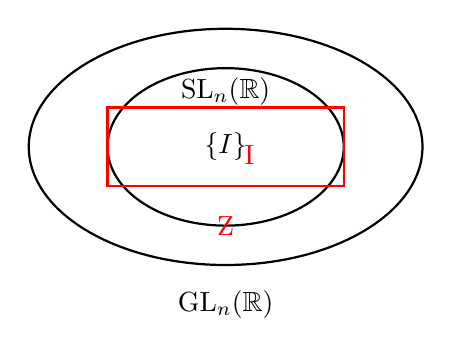
\begin{tikzpicture}
        % Draw the GL_n(R) and SL_n(R) sets
        \draw[thick] (0,0) ellipse (2.5cm and 1.5cm);
        \draw[thick] (0,0) ellipse (1.5cm and 1cm);
        \node at (0,0.7) {SL\(_n(\mathbb{R})\)};
        \node at (0,-2) {GL\(_n(\mathbb{R})\)};

        % Identity matrix
        \node at (0,0) {\(\{I\}\)};
        
        % Z subgroup
        \draw[thick, red] (-1.5,-0.5) rectangle (1.5,0.5);
        \node[red] at (0,-1) {Z};
        
        % Z intersect SL_n(R)
        \node[red] at (0.3,-0.1) {I};
    \end{tikzpicture}
    \end{center}
    
\end{exercise}
\newpage

%-----------------------------
\begin{exercise}{2.4.17} An automorphism of a group $G$ is an isomorphism \(G \rightarrow G\) from the group to itself. Fix \(g\in G\) and show that the function \(c_g: G \rightarrow G\) defined by \(c_g(x):=gxg^{-1}\) is an automorphism of $G$.

    \noindent\rule{\linewidth}{1pt}
    
    \section*{Solution}
    
    To show that \(c_g: G \rightarrow G\) defined by \(c_g(x) := gxg^{-1}\) is an automorphism of $G$, we need to verify two things:
    
    \begin{enumerate}
        \item \(c_g\) is a homomorphism.
        \item \(c_g\) is bijective.
    \end{enumerate}
    
    \subsection*{(1) \(c_g\) is a homomorphism}
    
    We need to show that for all \(x, y \in G\):
    \[
    c_g(xy) = c_g(x)c_g(y).
    \]
    
    \begin{proof} \(\)
    
    Let \(x, y \in G\). Then:
    \[
    c_g(xy) = g(xy)g^{-1}.
    \]
    
    Using the associative property of group multiplication:
    \[
    g(xy)g^{-1} = (gx)(yg^{-1}).
    \]
    
    Note that \(yg^{-1} = (g^{-1})^{-1}y = g^{-1}g y g^{-1}\). Thus:
    \[
    (gx)(yg^{-1}) = (gx)(g^{-1}g y g^{-1}) = gxg^{-1}gyg^{-1}.
    \]
    
    Simplifying further:
    \[
    gxg^{-1}gyg^{-1} = (gxg^{-1})(gyg^{-1}).
    \]
    
    Therefore:
    \[
    c_g(xy) = c_g(x)c_g(y).
    \]
    
    Thus, \(c_g\) is a homomorphism.
    
    \end{proof}
    
    \subsection*{(2) \(c_g\) is bijective}
    
    We need to show that \(c_g\) is both injective and surjective.
    
    \subsubsection*{Injectivity}
    
    To show injectivity, we need to show that if \(c_g(x) = c_g(y)\), then \(x = y\).
    
    \begin{proof} \(\)
    
    Suppose \(c_g(x) = c_g(y)\). Then:
    \[
    gxg^{-1} = gyg^{-1}.
    \]
    
    Multiplying both sides on the left by \(g^{-1}\) and on the right by \(g\), we get:
    \[
    g^{-1}(gxg^{-1})g = g^{-1}(gyg^{-1})g.
    \]
    
    Simplifying:
    \[
    x = y.
    \]
    
    Thus, \(c_g\) is injective.
    
    \end{proof}
    
    \subsubsection*{Surjectivity}
    
    To show surjectivity, we need to show that for every \(y \in G\), there exists an \(x \in G\) such that \(c_g(x) = y\).
    
    \begin{proof} \(\)
    
    Let \(y \in G\). We need to find \(x \in G\) such that:
    \[
    gxg^{-1} = y.
    \]
    
    Multiplying both sides on the left by \(g^{-1}\) and on the right by \(g\), we get:
    \[
    g^{-1}(gxg^{-1})g = g^{-1}yg.
    \]
    
    Simplifying:
    \[
    x = g^{-1}yg.
    \]
    
    Let \(x = g^{-1}yg\). Then:
    \[
    c_g(x) = c_g(g^{-1}yg) = g(g^{-1}yg)g^{-1} = y.
    \]
    
    Thus, \(c_g\) is surjective.
    
    \end{proof}
    
    \subsection*{Visualization}

    Visualization of the conjugation of \(x\) by \(g\):

    \begin{center}
    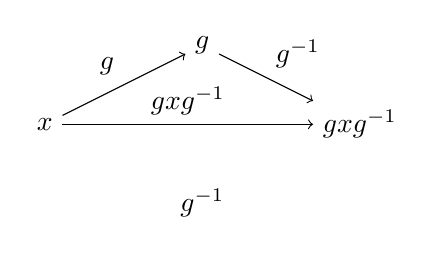
\begin{tikzpicture}
        \node (x) at (0,0) {\(x\)};
        \node (y) at (4,0) {\(gxg^{-1}\)};
        \node (g) at (2,1) {\(g\)};
        \node (g_inv) at (2,-1) {\(g^{-1}\)};
        
        \draw[->] (x) -- (y) node[midway, above] {\(gxg^{-1}\)};
        \draw[->] (x) -- (g) node[midway, above left] {\(g\)};
        \draw[->] (g) -- (y) node[midway, above right] {\(g^{-1}\)};
    \end{tikzpicture}
    \end{center}
    
    \subsection*{Conclusion}
    
    Since \(c_g\) is both a homomorphism and bijective, it is an automorphism of \(G\). Therefore, \(c_g: G \rightarrow G\) defined by \(c_g(x) := gxg^{-1}\) is an automorphism of \(G\).
    
\end{exercise}
\newpage

%-----------------------------
\begin{exercise}{2.5.3} The center of a group $G$ is the set \[Z(G) := \{a \in G \ | \ ag = ga \ \forall \ g \in G\}\] of elements which commute with every element of $G$. Show that \(Z(G)\) is a normal subgroup of $G$.

    \noindent\rule{\linewidth}{1pt}
    \section*{Solution}

    To show that \(Z(G)\), the center of a group \(G\), is a normal subgroup of \(G\), we need to verify two things:
    
    \begin{enumerate}
        \item \(Z(G)\) is a subgroup of \(G\).
        \item \(Z(G)\) is normal in \(G\).
    \end{enumerate}
    
    \subsection*{(1) \(Z(G)\) is a Subgroup of \(G\)}
    
    We will use the subgroup criteria to show that \(Z(G)\) is a subgroup of \(G\):
    
    \begin{itemize}
        \item The identity element \(e \in G\) is in \(Z(G)\) since \(eg = ge = g\) for all \(g \in G\).
        \item If \(a, b \in Z(G)\), then \(ab \in Z(G)\) because for any \(g \in G\),
        \[
        (ab)g = a(bg) = a(gb) = (ag)b = (ga)b = g(ab).
        \]
        Thus, \(ab\) commutes with every element of \(G\), so \(ab \in Z(G)\).
        \item If \(a \in Z(G)\), then \(a^{-1} \in Z(G)\) because for any \(g \in G\),
        \[
        a^{-1}g = a^{-1}(ga^{-1})a = (a^{-1}a)g(a^{-1}a)^{-1} = g(a^{-1}a)^{-1} = g(a^{-1}).
        \]
        Thus, \(a^{-1}\) commutes with every element of \(G\), so \(a^{-1} \in Z(G)\).
    \end{itemize}
    
    Since \(Z(G)\) contains the identity element, is closed under the group operation, and contains the inverses of its elements, \(Z(G)\) is a subgroup of \(G\).
    
    \subsection*{(2) \(Z(G)\) is Normal in \(G\)}
    
    We need to show that \(Z(G)\) is invariant under conjugation by any element of \(G\). That is, for any \(g \in G\) and \(a \in Z(G)\), we have \(gag^{-1} \in Z(G)\).
    
    \begin{proof} \(\)
    
    Let \(a \in Z(G)\). This means \(a\) commutes with every element of \(G\). Let \(g \in G\). We need to show that \(gag^{-1} \in Z(G)\). That is, \(gag^{-1}\) commutes with every element of \(G\).
    
    Let \(h \in G\). Then:
    \[
    (gag^{-1})h = ga(g^{-1}h) = g(ag^{-1}h) = g(g^{-1}ha) = (gg^{-1})ha = ha.
    \]
    
    Since \(a\) commutes with \(h\), we have:
    \[
    ha = ah.
    \]
    
    Thus:
    \[
    (gag^{-1})h = ha = ah = h(gag^{-1}).
    \]
    
    Therefore, \(gag^{-1}\) commutes with every element of \(G\), so \(gag^{-1} \in Z(G)\).
    
    \end{proof}
    
    \subsection*{Visualization}

    \begin{center}
    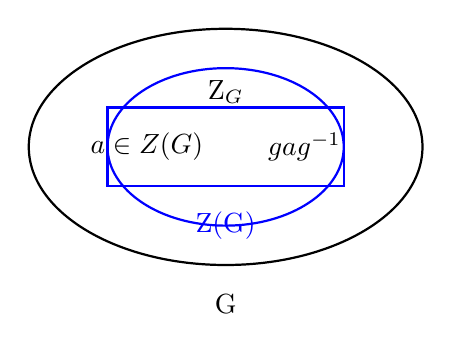
\begin{tikzpicture}
        % Draw the G and Z(G) sets
        \draw[thick] (0,0) ellipse (2.5cm and 1.5cm);
        \draw[thick, blue] (0,0) ellipse (1.5cm and 1cm);
        \node at (0,0.7) {Z\(_G\)};
        \node at (0,-2) {G};

        % Elements
        \node at (-1,0) {\(a \in Z(G)\)};
        \node at (1,0) {\(gag^{-1}\)};
        
        % Center subgroup
        \draw[thick, blue] (-1.5,-0.5) rectangle (1.5,0.5);
        \node[blue] at (0,-1) {Z(G)};
    \end{tikzpicture}
    \end{center}
    
    \subsection*{Conclusion}
    
    Since \(Z(G)\) is a subgroup of \(G\) and is invariant under conjugation by any element of \(G\), \(Z(G)\) is a normal subgroup of \(G\).
    
\end{exercise}
\newpage

%-----------------------------
\begin{exercise}{2.7.6} Denote the set of all automorphisms of \(G\) by \(\text{Aut}(G)\).
    \begin{enumerate}[label=\textbf{\alph*.}]
        \item Show that \(\text{Aut}(G)\) is a group, with the operation of composition of functions.
        \item Show that the function \(c:G\rightarrow \text{Aut}(G)\) defined by \(g \mapsto c_g\) is a homomorphism of groups.
        \item Show that the kernel of \(c\) is \(Z(G)\).
        \item The image of \(c\) is called the group of inner automorphisms of \(G\) and denoted \(\text{Inn}(G)\). Show that \(\text{Inn}(G) \cong G/Z(G)\).
    \end{enumerate}

    \noindent\rule{\linewidth}{1pt}
    
    \section*{Solution}
    
    \subsection*{a. \(\text{Aut}(G)\) is a Group}
    
    To show that \(\text{Aut}(G)\) is a group, we need to verify that it satisfies the group axioms with respect to the operation of composition of functions.
    
    \begin{proof} \( \)
    
    \begin{itemize}
        \item \textbf{Closure}: If \(\alpha, \beta \in \text{Aut}(G)\), then \(\alpha \circ \beta \in \text{Aut}(G)\). This is because the composition of two automorphisms is an automorphism.
        \item \textbf{Associativity}: Function composition is associative, so for any \(\alpha, \beta, \gamma \in \text{Aut}(G)\),
        \[
        (\alpha \circ \beta) \circ \gamma = \alpha \circ (\beta \circ \gamma).
        \]
        \item \textbf{Identity Element}: The identity automorphism \(id_G: G \to G\) defined by \(id_G(g) = g\) for all \(g \in G\) is in \(\text{Aut}(G)\) and serves as the identity element for composition:
        \[
        id_G \circ \alpha = \alpha \quad \text{and} \quad \alpha \circ id_G = \alpha \quad \text{for all } \alpha \in \text{Aut}(G).
        \]
        \item \textbf{Inverse Element}: For each \(\alpha \in \text{Aut}(G)\), there exists an inverse automorphism \(\alpha^{-1} \in \text{Aut}(G)\) such that
        \[
        \alpha \circ \alpha^{-1} = id_G \quad \text{and} \quad \alpha^{-1} \circ \alpha = id_G.
        \]
    \end{itemize}
    
    Therefore, \(\text{Aut}(G)\) is a group.
    
    \end{proof}
    
    \subsection*{b. The Function \(c: G \rightarrow \text{Aut}(G)\) is a Homomorphism}
    
    Define the function \(c: G \rightarrow \text{Aut}(G)\) by \(c_g(x) = gxg^{-1}\). We need to show that \(c\) is a homomorphism of groups.
    
    \begin{proof} \( \)
    
    Let \(g, h \in G\). We need to show that \(c_{gh} = c_g \circ c_h\). For any \(x \in G\),
    \[
    c_{gh}(x) = (gh)x(gh)^{-1}.
    \]
    
    On the other hand,
    \[
    (c_g \circ c_h)(x) = c_g(c_h(x)) = c_g(hxh^{-1}) = g(hxh^{-1})g^{-1} = (gh)x(h^{-1}g^{-1}) = (gh)x(gh)^{-1}.
    \]
    
    Thus,
    \[
    c_{gh}(x) = (c_g \circ c_h)(x) \quad \text{for all } x \in G.
    \]
    
    Therefore, \(c_{gh} = c_g \circ c_h\) and \(c\) is a homomorphism.
    
    \end{proof}
    
    \subsection*{c. The Kernel of \(c\) is \(Z(G)\)}
    
    The kernel of \(c\) consists of all elements \(g \in G\) such that \(c_g\) is the identity automorphism.
    
    \begin{proof} \( \)
    
    We need to show that
    \[
    \ker(c) = \{ g \in G \mid c_g(x) = x \text{ for all } x \in G \}.
    \]
    
    By definition,
    \[
    c_g(x) = gxg^{-1} = x \quad \text{for all } x \in G.
    \]
    
    This implies that \(g\) commutes with every element of \(G\). Hence,
    \[
    \ker(c) = Z(G) = \{ g \in G \mid gx = xg \text{ for all } x \in G \}.
    \]
    
    \end{proof}
    
    \subsection*{d. \(\text{Inn}(G) \cong G/Z(G)\)}
    
    The image of \(c\) is called the group of inner automorphisms of \(G\) and denoted \(\text{Inn}(G)\). We need to show that \(\text{Inn}(G) \cong G / Z(G)\).
    
    \begin{proof} \( \)
    
    Consider the homomorphism \(c: G \rightarrow \text{Inn}(G)\) defined by \(c_g(x) = gxg^{-1}\). By the First Isomorphism Theorem,
    \[
    G / \ker(c) \cong \text{Im}(c).
    \]
    
    From part (c), we know that \(\ker(c) = Z(G)\). Thus,
    \[
    G / Z(G) \cong \text{Im}(c) = \text{Inn}(G).
    \]
    
    Therefore,
    \[
    \text{Inn}(G) \cong G / Z(G).
    \]
    
    \end{proof}

    \subsection*{Visualization}

    Visualization of the automorphisms and inner automorphisms:

    \begin{center}
    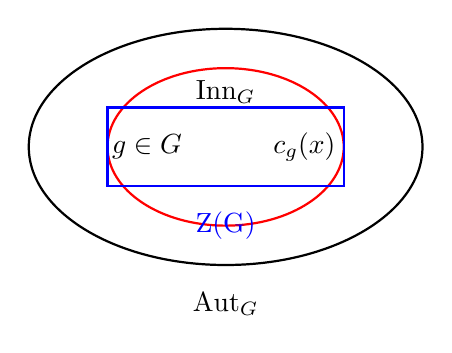
\begin{tikzpicture}
        % Draw the G, Aut(G) and Inn(G) sets
        \draw[thick] (0,0) ellipse (2.5cm and 1.5cm);
        \draw[thick, red] (0,0) ellipse (1.5cm and 1cm);
        \node at (0,0.7) {Inn\(_G\)};
        \node at (0,-2) {Aut\(_G\)};

        % Elements
        \node at (-1,0) {\(g \in G\)};
        \node at (1,0) {\(c_g(x)\)};
        
        % Center subgroup
        \draw[thick, blue] (-1.5,-0.5) rectangle (1.5,0.5);
        \node[blue] at (0,-1) {Z(G)};
    \end{tikzpicture}
    \end{center}
    
\end{exercise}
\newpage

%-----------------------------
\begin{exercise}{5} The purpose of this exercise is to compute the automorphism group of a finite cyclic group. Let \(G = \langle g \rangle\) be a finite cyclic group of order \(n\).
    \begin{enumerate}[label=\textbf{\alph*.}]
        \item Show that for any integer \(k \in \Z\), the function \(p_k: G \rightarrow G\) defined by \(p_k(x) := x^k\) defines a homomorphism from \(G\) to itself.
        \item Show that \(p_k\) is an isomorphism if and only if \(\gcd(k,n) = 1\).
        \item Show that \([k]_n \mapsto p_k\) defines an isomorphism of groups \(\Phi(n) \rightarrow \text{Aut}(G)\).
    \end{enumerate}
    
    \noindent\rule{\linewidth}{1pt}
    
    \section*{Solution}
    
    \subsection*{\textbf{a. \(p_k\) defines a homomorphism from \(G\) to itself}}
    
    Let \(G = \langle g \rangle\) be a finite cyclic group of order \(n\). We need to show that for any integer \(k \in \Z\), the function \(p_k: G \rightarrow G\) defined by \(p_k(x) := x^k\) is a homomorphism.
    
    \begin{proof} \( \)
    
    For any \(x, y \in G\), we have:
    \[
    p_k(xy) = (xy)^k.
    \]
    
    Since \(G\) is abelian (all cyclic groups are abelian), we can write:
    \[
    (xy)^k = x^k y^k.
    \]
    
    Thus,
    \[
    p_k(xy) = x^k y^k = p_k(x) p_k(y).
    \]
    
    Therefore, \(p_k\) is a homomorphism from \(G\) to itself.
    
    \end{proof}
    
    \subsection*{\textbf{b. \(p_k\) is an isomorphism if and only if \(\gcd(k, n) = 1\)}}
    
    We need to show that \(p_k\) is an isomorphism if and only if \(\gcd(k, n) = 1\).
    
    \begin{proof} \( \)
    
    \(p_k\) is an isomorphism if and only if it is bijective.
    
    \subsubsection*{Surjectivity}
    We first show that \(p_k\) is surjective. For any \(x \in G\), there exists some \(y \in G\) such that:
    \[
    p_k(y) = y^k = x.
    \]
    
    Since \(G\) is a finite cyclic group, this equation has a solution if and only if \(\gcd(k, n) = 1\). This is because for each \(x \in G\), \(x\) can be written as \(g^m\) for some \(m \in \{0, 1, \ldots, n-1\}\). Therefore, we need \(g^{km} = g^m\), which is possible if and only if \(k\) is relatively prime to \(n\).
    
    \subsubsection*{Injectivity}
    We now show that \(p_k\) is injective. Suppose \(p_k(x) = p_k(y)\) for \(x, y \in G\). This implies:
    \[
    x^k = y^k.
    \]
    
    Since \(G\) is cyclic, \(x\) and \(y\) can be written as \(x = g^a\) and \(y = g^b\) for some integers \(a, b\). Thus,
    \[
    (g^a)^k = (g^b)^k \implies g^{ak} = g^{bk} \implies ak \equiv bk \pmod{n}.
    \]
    
    Since \(\gcd(k, n) = 1\), we can divide both sides by \(k\) modulo \(n\), yielding:
    \[
    a \equiv b \pmod{n} \implies x = y.
    \]
    
    Thus, \(p_k\) is injective.
    
    Since \(p_k\) is both injective and surjective, it is an isomorphism if and only if \(\gcd(k, n) = 1\).
    
    \end{proof}
    
    \subsection*{\textbf{c. \([k]_n \mapsto p_k\) defines an isomorphism of groups \(\Phi(n) \rightarrow \text{Aut}(G)\)}}
    
    We need to show that the map \([k]_n \mapsto p_k\) defines an isomorphism from \(\Phi(n)\) to \(\text{Aut}(G)\).
    
    \begin{proof} \( \)
    
    Define the map \(\Phi: \Phi(n) \rightarrow \text{Aut}(G)\) by \(\Phi([k]_n) = p_k\).
    
    \subsubsection*{Homomorphism}
    We first show that \(\Phi\) is a homomorphism. For any \([k]_n, [m]_n \in \Phi(n)\), we have:
    \[
    \Phi([k]_n [m]_n) = \Phi([km]_n) = p_{km}.
    \]
    
    Since \(p_k \circ p_m = p_{km}\), we have:
    \[
    \Phi([k]_n) \Phi([m]_n) = p_k p_m = p_{km} = \Phi([km]_n).
    \]
    
    Thus, \(\Phi\) is a homomorphism.
    
    \subsubsection*{Injectivity}
    We now show that \(\Phi\) is injective. Suppose \(\Phi([k]_n) = \Phi([m]_n)\). This implies \(p_k = p_m\), meaning \(x^k = x^m\) for all \(x \in G\).
    
    Since \(G\) is cyclic, this implies \(k \equiv m \pmod{n}\). Therefore, \([k]_n = [m]_n\) in \(\Phi(n)\), showing that \(\Phi\) is injective.
    
    \subsubsection*{Surjectivity}
    Finally, we show that \(\Phi\) is surjective. For any automorphism \(\psi \in \text{Aut}(G)\), there exists an integer \(k\) such that \(\psi = p_k\) because \(\psi(g) = g^k\) for some \(k \in \{1, 2, \ldots, n-1\}\).
    
    Since \(\psi\) is an automorphism, \(\gcd(k, n) = 1\). Therefore, \([k]_n \in \Phi(n)\) and \(\Phi([k]_n) = p_k = \psi\).
    
    Thus, \(\Phi\) is surjective.
    
    Since \(\Phi\) is a bijective homomorphism, it is an isomorphism. Therefore, \([k]_n \mapsto p_k\) defines an isomorphism of groups \(\Phi(n) \rightarrow \text{Aut}(G)\).
    
    \end{proof}
    
\begin{figure}[h!]
    \centering
    \begin{tikzpicture}
        % Define the style for cyclic nodes
        \tikzstyle{cycnode}=[circle, draw, minimum size=1cm, inner sep=0pt]
        
        % Define the nodes
        \node[cycnode] (e) at (0,0) {$e$};
        \node[cycnode] (g1) at (2,2) {$g$};
        \node[cycnode] (g2) at (4,0) {$g^2$};
        \node[cycnode] (g3) at (2,-2) {$g^3$};
        \node (gn) at (6,0) {$\ldots$};
        
        % Define the arrows for p_k
        \draw[->] (e) edge[bend left=20] node[above left] {$p_k$} (g1);
        \draw[->] (g1) edge[bend left=20] node[above right] {$p_k$} (g2);
        \draw[->] (g2) edge[bend left=20] node[below right] {$p_k$} (g3);
        \draw[->] (g3) edge[bend left=20] node[below left] {$p_k$} (gn);
        
        % Define the commutative diagram for isomorphism
        \node (phi) at (2,-4) {$\Phi(n)$};
        \node (aut) at (6,-4) {$\text{Aut}(G)$};
        
        \draw[->] (phi) -- node[above] {$\Phi$} (aut);
    \end{tikzpicture}
    \caption{Visualization of Homomorphism and Isomorphism}
    \label{fig:homomorphism_isomorphism}
\end{figure}

\end{exercise}
\newpage

%-----------------------------
\begin{exercise}{3.1.9} Show that the direct product of \(A\times B\) is abelian if and only if $A$ and $B$ are abelian.
    
    \noindent\rule{\linewidth}{1pt}

    \section*{Solution}

    Let \(A\) and \(B\) be groups, and consider their direct product \(A \times B\). We will show that \(A \times B\) is abelian if and only if both \(A\) and \(B\) are abelian.

    \subsection*{Necessity: If \(A \times B\) is abelian, then \(A\) and \(B\) are abelian}

    Suppose \(A \times B\) is abelian. This means that for any \((a_1, b_1), (a_2, b_2) \in A \times B\),
    \[
    (a_1, b_1) (a_2, b_2) = (a_2, b_2) (a_1, b_1).
    \]

    The group operation in \(A \times B\) is defined component-wise. Therefore,
    \[
    (a_1 a_2, b_1 b_2) = (a_2 a_1, b_2 b_1).
    \]

    This implies
    \[
    a_1 a_2 = a_2 a_1 \quad \text{and} \quad b_1 b_2 = b_2 b_1 \quad \text{for all } a_1, a_2 \in A \text{ and } b_1, b_2 \in B.
    \]

    Therefore, both \(A\) and \(B\) are abelian.

    \subsection*{Sufficiency: If \(A\) and \(B\) are abelian, then \(A \times B\) is abelian}

    Suppose \(A\) and \(B\) are abelian. This means that for any \(a_1, a_2 \in A\),
    \[
    a_1 a_2 = a_2 a_1,
    \]
    and for any \(b_1, b_2 \in B\),
    \[
    b_1 b_2 = b_2 b_1.
    \]

    Consider any two elements \((a_1, b_1), (a_2, b_2) \in A \times B\). The group operation in \(A \times B\) is defined component-wise, so
    \[
    (a_1, b_1) (a_2, b_2) = (a_1 a_2, b_1 b_2).
    \]

    Since \(A\) and \(B\) are abelian,
    \[
    a_1 a_2 = a_2 a_1 \quad \text{and} \quad b_1 b_2 = b_2 b_1.
    \]

    Therefore,
    \[
    (a_1 a_2, b_1 b_2) = (a_2 a_1, b_2 b_1) = (a_2, b_2) (a_1, b_1).
    \]

    This shows that
    \[
    (a_1, b_1) (a_2, b_2) = (a_2, b_2) (a_1, b_1) \quad \text{for all } (a_1, b_1), (a_2, b_2) \in A \times B.
    \]

    Thus, \(A \times B\) is abelian.

    \subsection*{Visualization}

    Visualization of the direct product \(A \times B\):

    \begin{center}
    \begin{tikzpicture}
        % Axes
        \draw[<->] (0,4) node (yaxis) [above] {$B$}
            |- (4,0) node (xaxis) [right] {$A$};
        
        % Elements in A and B
        \foreach \x in {1,2,3}
            \foreach \y in {1,2,3}
                \node[draw, circle, inner sep=1pt, fill=black] at (\x,\y) {};

        % Labels
        \node at (0.5,3.5) {B};
        \node at (3.5,0.5) {A};
    \end{tikzpicture}
    \end{center}
    
    \subsection*{Conclusion}

    The direct product \(A \times B\) is abelian if and only if both \(A\) and \(B\) are abelian.

\end{exercise}
\newpage

%-----------------------------
\begin{exercise}{3.1.14} Show that \(\Z_4 \times \Z_4\) is not isomorphic to \(\Z_4 \times \Z_2 \times \Z_2\). (See hint in book.)
    
    \noindent\rule{\linewidth}{1pt}

    \section*{Solution}

    To show that \(\Z_4 \times \Z_4\) is not isomorphic to \(\Z_4 \times \Z_2 \times \Z_2\), we will count the number of elements of order 4 in each group and show that they differ.

    \subsection*{Elements of Order 4 in \(\Z_4 \times \Z_4\)}

    The group \(\Z_4 \times \Z_4\) consists of pairs \((a, b)\) where \(a, b \in \Z_4\). An element \((a, b) \in \Z_4 \times \Z_4\) has order 4 if and only if the least common multiple of the orders of \(a\) and \(b\) is 4. The possible orders of elements in \(\Z_4\) are 1, 2, and 4.

    \begin{itemize}
        \item For an element \((a, b)\) to have order 4, either \(a\) or \(b\) must have order 4, and the other must have order 1 or 4.
    \end{itemize}

    \subsubsection*{Case 1: \(a\) has order 4}

    If \(a\) has order 4, then \(a\) can be 1 element (\(a = 1\) or \(a = 3\)) because there are 2 elements of order 4 in \(\Z_4\).

    \begin{itemize}
        \item \(b\) must have order 1 or 4:
            \begin{itemize}
                \item There are 2 elements of order 4 (\(b = 1\) or \(b = 3\)).
                \item There is 1 element of order 1 (\(b = 0\)).
            \end{itemize}
    \end{itemize}

    Therefore, for each \(a\) of order 4, there are \(2 + 1 = 3\) choices for \(b\), and there are 2 possible values for \(a\), resulting in \(2 \times 3 = 6\) elements.

    \subsubsection*{Case 2: \(b\) has order 4}

    This is similar to Case 1, and it also gives 6 elements.

    Therefore, the total number of elements of order 4 in \(\Z_4 \times \Z_4\) is \(6 + 6 = 12\).

    \subsection*{Elements of Order 4 in \(\Z_4 \times \Z_2 \times \Z_2\)}

    The group \(\Z_4 \times \Z_2 \times \Z_2\) consists of triples \((a, b, c)\) where \(a \in \Z_4\) and \(b, c \in \Z_2\). An element \((a, b, c) \in \Z_4 \times \Z_2 \times \Z_2\) has order 4 if and only if \(a\) has order 4.

    \begin{itemize}
        \item There are 2 elements in \(\Z_4\) with order 4 (\(a = 1\) or \(a = 3\)).
        \item Each element \(b \in \Z_2\) has order 2 or 1, and similarly for \(c \in \Z_2\). There are \(2 \times 2 = 4\) combinations of \(b\) and \(c\).
    \end{itemize}

    Therefore, for each \(a\) of order 4, there are 4 choices for \((b, c)\), resulting in \(2 \times 4 = 8\) elements of order 4.

    \subsection*{Conclusion}

    The number of elements of order 4 in \(\Z_4 \times \Z_4\) is 12, while the number of elements of order 4 in \(\Z_4 \times \Z_2 \times \Z_2\) is 8. Since the number of elements of order 4 differs in the two groups, they cannot be isomorphic.

    \subsection*{Visualization}

    Visualization of the elements of order 4:

    \begin{center}
    \begin{tikzpicture}
        % Axes for Z4 x Z4
        \draw[<->] (0,4) node (yaxis1) [above] {\(Z_4\)}
            |- (4,0) node (xaxis1) [right] {\(Z_4\)};
        \foreach \x in {1,2,3}
            \foreach \y in {1,2,3}
                \node[draw, circle, inner sep=1pt, fill=black] at (\x,\y) {};

        % Axes for Z4 x Z2 x Z2
        \draw[<->] (6,4) node (yaxis2) [above] {\(Z_2\)}
            |- (10,0) node (xaxis2) [right] {\(Z_4 \times Z_2\)};
        \foreach \x in {7,8,9}
            \foreach \y in {1,2,3}
                \node[draw, circle, inner sep=1pt, fill=black] at (\x,\y) {};
    \end{tikzpicture}
    \end{center}

\end{exercise}
\newpage

%-----------------------------
\begin{exercise}{3.1.15} Let \(K_1\) be a normal subgroup of \(G_1\), and \(K_2\) a normal subgroup of \(G_2\). Show that \(K_1 \times K_2\) is a normal subgroup of \(G_1 \times G_2\), and that \[(G_1 \times G_2)/(K_1\times K_2) \cong (G_1/K_1) \times (G_2/K_2)\]
    
    \noindent\rule{\linewidth}{1pt}
    
    \section*{Solution}
    
    \subsection*{Normality of \(K_1 \times K_2\) in \(G_1 \times G_2\)}
    
    Let \(K_1\) be a normal subgroup of \(G_1\), and \(K_2\) be a normal subgroup of \(G_2\). We want to show that \(K_1 \times K_2\) is a normal subgroup of \(G_1 \times G_2\).
    
    \begin{proof} \( \)
    
    Consider any element \((g_1, g_2) \in G_1 \times G_2\) and any element \((k_1, k_2) \in K_1 \times K_2\). We need to show that:
    \[
    (g_1, g_2)(k_1, k_2)(g_1, g_2)^{-1} \in K_1 \times K_2.
    \]
    
    Calculate the product:
    \[
    (g_1, g_2)(k_1, k_2)(g_1, g_2)^{-1} = (g_1 k_1, g_2 k_2) (g_1^{-1}, g_2^{-1}) = (g_1 k_1 g_1^{-1}, g_2 k_2 g_2^{-1}).
    \]
    
    Since \(K_1\) is normal in \(G_1\), we have \(g_1 k_1 g_1^{-1} \in K_1\). Similarly, since \(K_2\) is normal in \(G_2\), we have \(g_2 k_2 g_2^{-1} \in K_2\).
    
    Therefore:
    \[
    (g_1 k_1 g_1^{-1}, g_2 k_2 g_2^{-1}) \in K_1 \times K_2.
    \]
    
    Thus, \(K_1 \times K_2\) is a normal subgroup of \(G_1 \times G_2\).
    
    \end{proof}
    
    \subsection*{Isomorphism \((G_1 \times G_2)/(K_1 \times K_2) \cong (G_1/K_1) \times (G_2/K_2)\)}
    
    We want to show that:
    \[
    (G_1 \times G_2)/(K_1 \times K_2) \cong (G_1/K_1) \times (G_2/K_2).
    \]
    
    Define the map \(\phi: (G_1 \times G_2) \rightarrow (G_1/K_1) \times (G_2/K_2)\) by:
    \[
    \phi(g_1, g_2) = (g_1 K_1, g_2 K_2).
    \]
    
    \begin{proof} \( \)
    
    First, we show that \(\phi\) is a homomorphism. For any \((g_1, g_2), (h_1, h_2) \in G_1 \times G_2\):
    \[
    \phi((g_1, g_2)(h_1, h_2)) = \phi(g_1 h_1, g_2 h_2) = (g_1 h_1 K_1, g_2 h_2 K_2).
    \]
    
    Since \(g_1 h_1 K_1 = (g_1 K_1)(h_1 K_1)\) and \(g_2 h_2 K_2 = (g_2 K_2)(h_2 K_2)\), we have:
    \[
    (g_1 h_1 K_1, g_2 h_2 K_2) = (g_1 K_1, g_2 K_2)(h_1 K_1, h_2 K_2) = \phi(g_1, g_2)\phi(h_1, h_2).
    \]
    
    Thus, \(\phi\) is a homomorphism.
    
    Next, we show that \(\phi\) is surjective. For any \((g_1 K_1, g_2 K_2) \in (G_1/K_1) \times (G_2/K_2)\), there exist \(g_1 \in G_1\) and \(g_2 \in G_2\) such that:
    \[
    \phi(g_1, g_2) = (g_1 K_1, g_2 K_2).
    \]
    
    Therefore, \(\phi\) is surjective.
    
    Finally, we show that \(\ker(\phi) = K_1 \times K_2\). For any \((g_1, g_2) \in G_1 \times G_2\):
    \[
    \phi(g_1, g_2) = (K_1, K_2) \implies g_1 K_1 = K_1 \text{ and } g_2 K_2 = K_2 \implies g_1 \in K_1 \text{ and } g_2 \in K_2.
    \]
    
    Thus, \(\ker(\phi) = K_1 \times K_2\).
    
    By the First Isomorphism Theorem, we have:
    \[
    (G_1 \times G_2)/(K_1 \times K_2) \cong \phi(G_1 \times G_2) = (G_1/K_1) \times (G_2/K_2).
    \]
    
    \end{proof}

    \subsection*{Visualization}

    Visualization of the isomorphism:

    \begin{center}
    \begin{tikzpicture}
        % Axes for G1 x G2
        \draw[<->] (0,4) node (yaxis1) [above] {\(G_2\)}
            |- (4,0) node (xaxis1) [right] {\(G_1\)};
        \foreach \x in {1,2,3}
            \foreach \y in {1,2,3}
                \node[draw, circle, inner sep=1pt, fill=black] at (\x,\y) {};

        % Normal subgroups
        \foreach \x in {1,2,3}
            \node[draw, rectangle, inner sep=1pt, fill=blue] at (\x,2) {};
        \foreach \y in {1,2,3}
            \node[draw, rectangle, inner sep=1pt, fill=blue] at (2,\y) {};

        % Axes for G1/K1 x G2/K2
        \draw[<->] (6,4) node (yaxis2) [above] {\(G_2/K_2\)}
            |- (10,0) node (xaxis2) [right] {\(G_1/K_1\)};
        \foreach \x in {7,8,9}
            \foreach \y in {1,2,3}
                \node[draw, circle, inner sep=1pt, fill=black] at (\x,\y) {};
    \end{tikzpicture}
    \end{center}
    
\end{exercise}
\newpage

\end{document}
